
\begin{center}
	\Huge
	Parallelforskydning af grafer.
\end{center}

\section*{Parallelforskydning}
\stepcounter{section}

Vi kan parallelforskyde grafer for funktioner på to forskellige måder. Vi kan lægge et tal til funktionsforskriften for på denne måde at parallelforskyde grafen langs $y$-aksen. Og vi kan lægge et tal til $x$-værdien og parallelforskyde grafen for funktion langs $x$-aksen. 

\begin{setn}[Parallelforskydning]
	Lad $f$ være en funktion. Grafen for $f$ kan parallelforskydes med $b$ op langs $y$-aksen ved at lægge $b$
	til funktionsforskriften som
	\begin{align*}
		f(x) + b.
	\end{align*}
	Grafen for $f$ kan parallelforskydes med $a$ til venstre langs $x$-aksen ved at lægge $a$ til 
	funktionsargumentet som
	\begin{align*}
		f(x + a).
	\end{align*}
	En parallelforskydning både langs $x$-aksen og $y$-aksen kan altså skrives
	\begin{align*}
		f(x + a) + b.
	\end{align*}
\end{setn}
Vi kan se en parallelforskydning langs $y$-aksen på Figur \ref{fig:yparallel} og en parallelforskydning
langs $x$-aksen på Figur \ref{fig:xparallel}.
\begin{figure}[H]
	\centering
	\begin{minipage}{0.48\textwidth}
		\centering
		\resizebox{0.98\textwidth}{!}{
		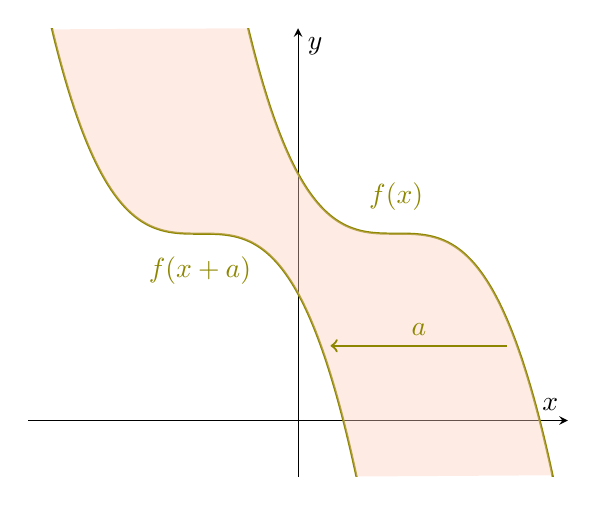
\begin{tikzpicture}
		\begin{axis}[
		axis lines = center,
		xmin = -5.5, xmax = 5.5,
		ymin = -1.5, ymax = 10.5,
		xlabel = $x$, ylabel = $y$, 
		ticks = none,
		]
			\addplot[color = olive, thick, samples = 400, domain = -5.5:5.5] {-1/5*(x-2)^3 +  5 };
			\addplot[color = olive, thick, samples = 400, domain = -5.5:5.5] {-1/5*(x+2)^3 +  5 };
			\fill[Melon!40, opacity = 0.4, variable = \x ]
			plot[domain = -1.018:5.19125, samples = 400] (axis cs: \x ,{-1/5*( \x - 2)^3 + 5})
			--
			plot[domain = 1.19125:-5.018, samples = 400] (axis cs: \x ,{-1/5*( \x + 2 )^3 + 5}) 
			--
			cycle;
			\draw[->, color = olive, thick] (axis cs: 4.6621-0.4, 2) -- (axis cs: 0.6621,2)
			 node[midway, anchor = south] {$a$};
			\node[color = olive] at (axis cs: 2,6) {$f(x)$};
			\node[color = olive] at (axis cs: -2,4) {$f(x+a)$};
		\end{axis}
		\end{tikzpicture}
		}
		\caption{Vandret parallelforskydning (langs $x$-aksen).}
		\label{fig:xparallel}
	\end{minipage}
	\begin{minipage}{0.48\textwidth}
		\centering
		\resizebox{0.98\textwidth}{!}{
		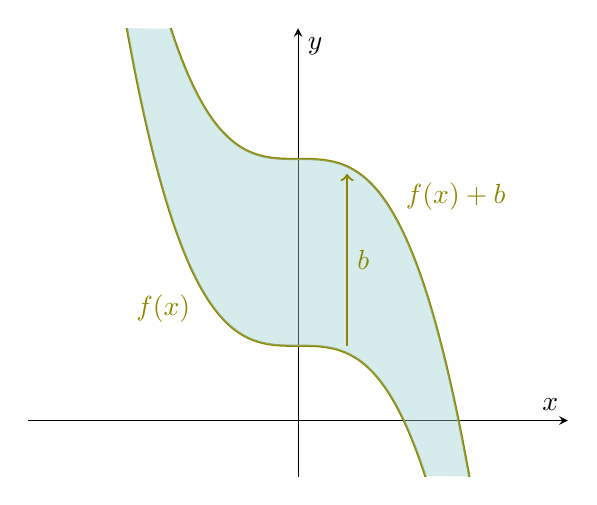
\begin{tikzpicture}
		\begin{axis}[
		axis lines = center,
		xmin = -5.5, xmax = 5.5,
		ymin = -1.5, ymax = 10.5,
		xlabel = $x$, ylabel = $y$, 
		ticks = none
		]
			\addplot[color = olive, thick, samples = 400, domain = -5.5:5.5] {-1/5*(x)^3 +  2 };
			\addplot[color = olive, thick, samples = 400, domain = -5.5:5.5] {-1/5*(x)^3 +  7 };
			\fill[teal!40, opacity = 0.4, variable = \x ]
			plot[domain = -3.48977:2.59625, samples = 400] (axis cs: \x ,{-1/5*( \x )^3 + 2})
			--
			plot[domain = 3.48977:-2.59625, samples = 400] (axis cs: \x ,{-1/5*( \x )^3 + 7})  
			--
			cycle;
			\draw[thick, color = olive, ->] (axis cs: 1,9/5+0.2) -- (axis cs: 1,9/5 + 5-0.2)
			node[midway, anchor = west] {$b$};
			\node[color = olive, anchor = east] at (axis cs: -2,3) {$f(x)$};
			\node[color = olive, anchor = west] at (axis cs: 2,6) {$f(x) + b$};
		\end{axis}
		\end{tikzpicture}
		}
		\caption{Lodret parallelforskydning (langs $y$-aksen).}
		\label{fig:yparallel}
	\end{minipage}
\end{figure}
\begin{exa}
	Vi betragter funktionen $f(x) = x^2$. Vi kan parallelforskyde $f$ langs $x$-aksen og få
	\begin{align*}
		f(x + 2) = (x + 2)^2.
	\end{align*}
	Vi kan også parallelforskyde langs $y$-aksen og få
	\begin{align*}
		f(x) + 3 = x^2 + 3.
	\end{align*}
	Vi kan samle disse parallelforskydninger og få
	\begin{align*}
		f(x+2) +3 = (x+2)^2 + 3.
	\end{align*}
	Vi kan se disse funktioner tegnet på Figur \ref{fig:treforskydning}.
	\begin{figure}[H]
		\centering
		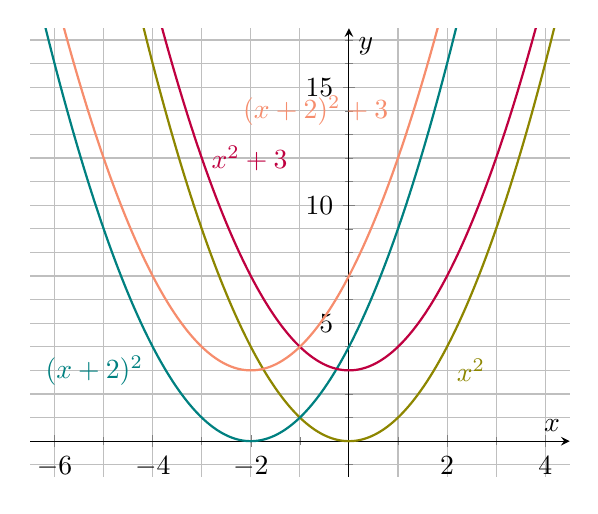
\begin{tikzpicture}
		\begin{axis}[
		axis lines = center, 
		xmin = -6.5, xmax = 4.5,
		ymin = -1.5, ymax = 17.5,
		xtick = {-6,-4,...,2,4},
		ytick = {-5,0,...,15,20},
		minor x tick num = 1,
		minor y tick num = 4,
		grid = both,
		xlabel = $x$,
		ylabel = $y$,
		]
			\addplot[color = olive, thick, domain = -7:5, samples = 400] {x^2};
			\addplot[color = teal, thick, domain = -7:5,samples = 400] {(x+2)^2};
			\addplot[color = purple, thick, domain = -7:5,samples = 400] {x^2+3};
			\addplot[color = Melon, thick, domain = -7:5,samples = 400] {(x+2)^2+3};
			\node[color = olive, anchor = west] at (axis cs: 2,3) {$x^2$};
			\node[color = teal, anchor = east] at (axis cs: -4,3) {$(x+2)^2$};
			\node[color = purple, anchor = west] at (axis cs: -3,12) {$x^2 + 3$};
			\node[color = Melon, anchor = east] at (axis cs: 1,14) {$(x+2)^2+3$};
		\end{axis}
		\end{tikzpicture}
		\caption{Parallelforskydninger af grafen for funktionen $f(x) = x^2$.}
		\label{fig:treforskydning}
	\end{figure}
\end{exa}

\newpage

\subsection*{Opgave 1}
Udfyld følgende tabel og skitser de fem grafer på koordinatsystemet.
\begin{center}
	\begin{table}[H]
	\centering
	\rowcolors{2}{Melon!40}{white}
	\begin{tabular}{c|ccccc}
	$x$ & $(x-2)^2$ & $(x-1)^2$ & $x^2$ & $(x+1)^2 $ & $(x+2)^2$  \\
	\hline
	$-4$ &&&&& \\
	$-3$ &&&&& \\
	$-2$ &&&&& \\
	$-1$ &&&&& \\
	$0$ &&&&& \\
	$1$ &&&&& \\
	$2$ &&&&& \\
	$3$ &&&&& \\
	$4$ &&&&& 
	\end{tabular}
	\end{table}
	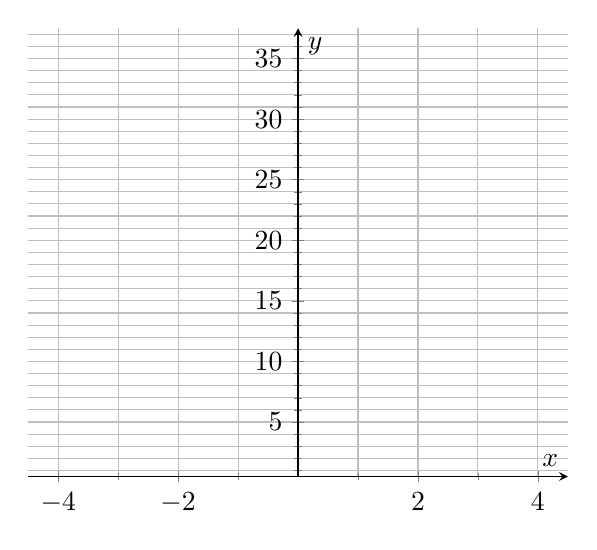
\begin{tikzpicture}
	\begin{axis}[
	axis lines = center, 
	xmin = -4.5,xmax = 4.5,
	ymin = 0.5, ymax = 37.5,
	xtick = {-6,-4,...,4,6},
	ytick = {-5,0,...,30,35,40},
	minor x tick num = 1, 
	minor y tick num = 4,
	grid = both,
	xlabel = $x$, ylabel = $y$,
	]
	
	\end{axis}
	\end{tikzpicture}
\end{center}
Kan du gennemskue, hvad der sker med grafen, hvis vi lægger et tal til $x$-værdien som det eksempelvis sker for $x^2 \to (x+1)^2$.

\newpage
\subsection*{Opgave 2}
\begin{center}
	\begin{table}[H]
	\centering
	\rowcolors{2}{Melon!40}{white}
	\begin{tabular}{c|ccc}
	$x$ & $x^2$ & $x^2 + 3$ & $x^2 + 6$  \\
	\hline
	$-4$ &&& \\
	$-3$ &&& \\
	$-2$ &&& \\
	$-1$ &&& \\
	$0$ &&& \\
	$1$ &&& \\
	$2$ &&& \\
	$3$ &&& \\
	$4$ &&& 
	\end{tabular}
	\end{table}
	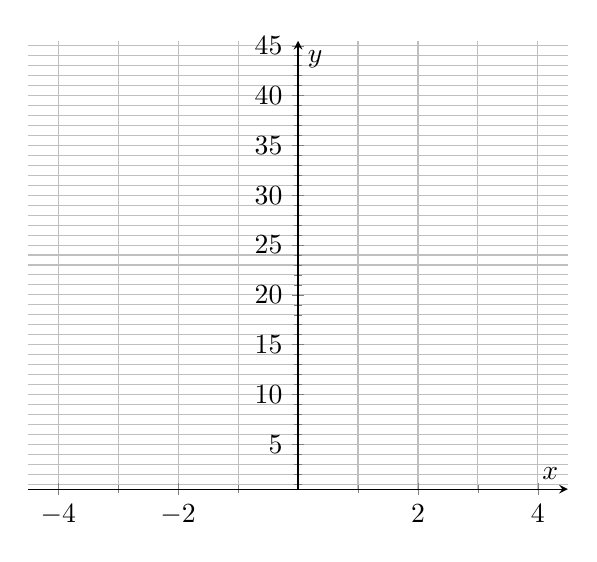
\begin{tikzpicture}
	\begin{axis}[
	axis lines = center, 
	xmin = -4.5,xmax = 4.5,
	ymin = 0.5, ymax = 45.5,
	xtick = {-6,-4,...,4,6},
	ytick = {-5,0,...,40,45},
	minor x tick num = 1, 
	minor y tick num = 4,
	grid = both,
	xlabel = $x$, ylabel = $y$, 
	]
	
	\end{axis}
	\end{tikzpicture}
\end{center}
Kan du gennemskue, hvad der sker med grafen, hvis vi lægger et tal til $y$-værdien, som det eksempelvis er tilfældet med $x^2 + 3 \to x^2 + 6$?

\newpage
\subsection*{Opgave 3}
\begin{enumerate}[label=\roman*)]
	\item Parallelforskyd grafen for $f(x) = x^2$ langs $x$-aksen så den går gennem punktet $(2,49)$.
	\item Parallelforskyd grafen for $f(x) = x^2$ langs $y$-aksen, så den går gennem punktet $(4,20)$.
	\item Parallelforskyd grafen for $f(x) = 10x - 5$ langs $x$-aksen, så den går gennem punktet $(5,-5)$.
	\item Parallelforskyd grafen for $f(x) = 2^x$ langs $x$-aksen, så den går gennem punktet $(5,4)$
\end{enumerate}

\subsection*{Opgave 4}
Opskriv forskriften for følgende grafer og parallelforskyd derefter en af graferne henholdsvis vandret og lodret, så de bliver kontinuerte (sammenhængene) funktioner.
\begin{center}
	\resizebox{0.48\textwidth}{!}{
	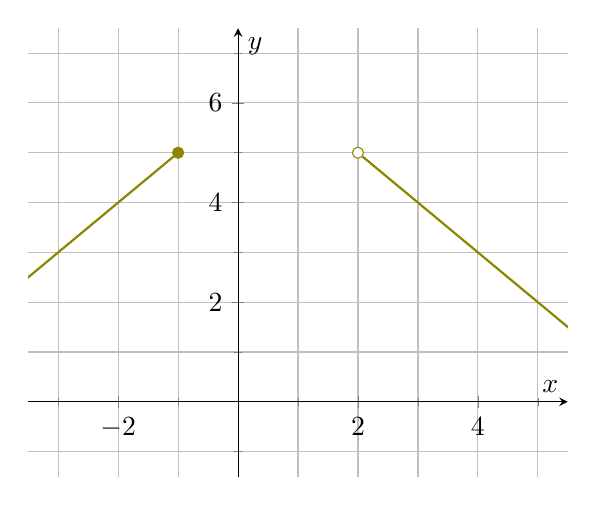
\begin{tikzpicture}
	\begin{axis}[
	axis lines = center, 
	xmin = -3.5, xmax = 5.5,
	ymin = -1.5, ymax = 7.5,
	xlabel = $x$, ylabel = $y$,
	xtick = {-4,-2,...,6,8},
	ytick = {-4,-2,...,8,10},
	minor tick num = 1, 
	grid = both,
	]
		\addplot[color = olive, thick, domain = -5:-1] {x + 6};
		\addplot[color = olive, thick, domain = 2:6] {-x + 7};
		\filldraw[color = olive] (axis cs: -1,5) circle (2pt);
		\filldraw[color = white] (axis cs: 2,5) circle (2pt);
		\draw[color = olive] (axis cs: 2,5) circle (2pt);
	\end{axis}
	\end{tikzpicture}
	}
	\resizebox{0.48\textwidth}{!}{
	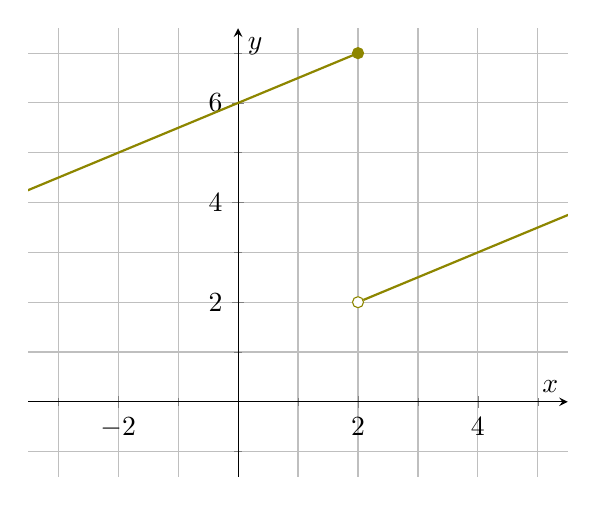
\begin{tikzpicture}
	\begin{axis}[
	axis lines = center, 
	xmin = -3.5, xmax = 5.5,
	ymin = -1.5, ymax = 7.5,
	xlabel = $x$, ylabel = $y$,
	xtick = {-4,-2,...,6,8},
	ytick = {-4,-2,...,8,10},
	minor tick num = 1, 
	grid = both,
	]
		\addplot[color = olive, thick, domain = -5:2] {0.5*x + 6};
		\addplot[color = olive, thick, domain = 2:6] {0.5*x + 1};
		\filldraw[color = olive] (axis cs: 2,7) circle (2pt);
		\filldraw[color = white] (axis cs: 2,2) circle (2pt);
		\draw[color = olive] (axis cs: 2,2) circle (2pt);
	\end{axis}
	\end{tikzpicture}
	}
\end{center}

\newpage
\subsection*{Opgave 5}
I følgende koordinatsystem ses graferne for funktionerne $f:]-\infty,-1[ \to \mathbb{R}$ og 
$g:[2,+\infty[ \to \mathbb{R}$ givet ved
\begin{align*}
	f(x) &= -2x + 2,\\
	g(x) &= x^2 - 6x + 10.
\end{align*}
Forskyd grafen for $g$, så $f$ og $g$ til sammen danner en kontinuert funktion. Tegn denne funktion i Maple og undersøg, om du har forskudt grafen korrekt. 

\begin{center}
	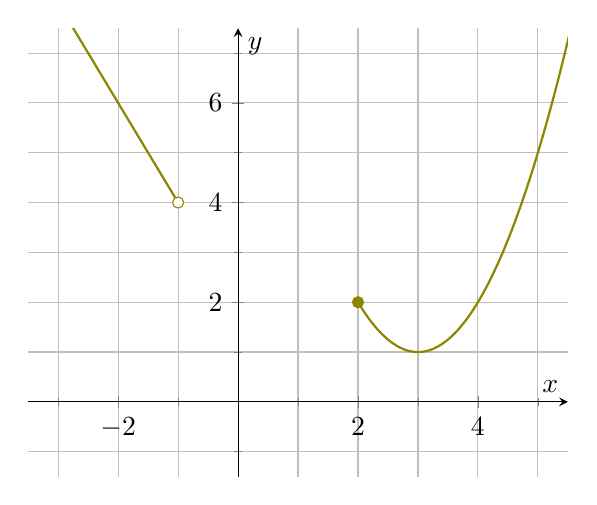
\begin{tikzpicture}
	\begin{axis}[
	axis lines = center, 
	xmin = -3.5, xmax = 5.5,
	ymin = -1.5, ymax = 7.5,
	xlabel = $x$, ylabel = $y$,
	xtick = {-4,-2,...,6,8},
	ytick = {-4,-2,...,8,10},
	minor tick num = 1, 
	grid = both,
	]
		\addplot[color = olive, thick, domain = -5:-1] {-2*x + 2};
		\addplot[color = olive, thick, domain = 2:6, samples = 400] {x^2 - 6*x + 10};
		\filldraw[color = olive] (axis cs: 2,2) circle (2pt);
		\filldraw[color = white] (axis cs: -1,4) circle (2pt);
		\draw[color = olive] (axis cs: -1,4) circle (2pt);
	\end{axis}
	\end{tikzpicture}
\end{center}

\subsection*{Opgave 6}
En funktion $f$ siges at være \textit{lige}, hvis det for alle $x \in \textnormal{Dm}(f)$ gælder, at
\begin{align*}
	f(x) = f(-x).
\end{align*}
Modsat siges $f$ at være \textit{ulige}, hvis det gælder, at
\begin{align*}
	f(x) = -f(-x).
\end{align*}
\begin{enumerate}[label=\roman*)]
	\item Afgør, om funktionerne $\cos(x)$ og $\sin(x)$ er ulige eller lige funktioner. 
	\item Parallelforskyd $\cos(x)$, så det bliver den omvendte funktionstype. Tegn eventuelt funktionen i 
	GeoGebra og anvend en skyder.
	\item Parallelforskyd $\sin(x)$, så det bliver den omvendte funktionstype. Tegn eventuelt funktionen i 
	GeoGebra og anvend en skyder.
\end{enumerate}